\documentclass{article}
\usepackage[margin=1.25in]{geometry}
\usepackage{graphicx, hyperref, float, multicol, pdflscape}
\usepackage[backend=bibtex, natbib=true]{biblatex}
\addbibresource{references/refs.bib}

\usepackage{color}
\newcommand{\hh}[1]{{\color{magenta} #1}}


\title{gravicom - a web-based tool for community detection in networks}
\author{Andrea J. Kaplan}

\begin{document}

\maketitle
\section{Background}
\subsection{Networks}
\subsection{Visualization}
\subsection{Layout Algorithms}

\section{User Interface}
\subsection{Design and Functionality}

Before discussing gravicom's performance and use on example datasets, we give a brief overview of the components and functionality that make up the tool.



\subsubsection{Description}

The gravicom interface is comprised of five main parts,
\begin{enumerate}
\item Control panel
\item Data management
\item Connection table 
\item Graph display
\item Tabset.
\end{enumerate}

\begin{figure}[H]
\centering
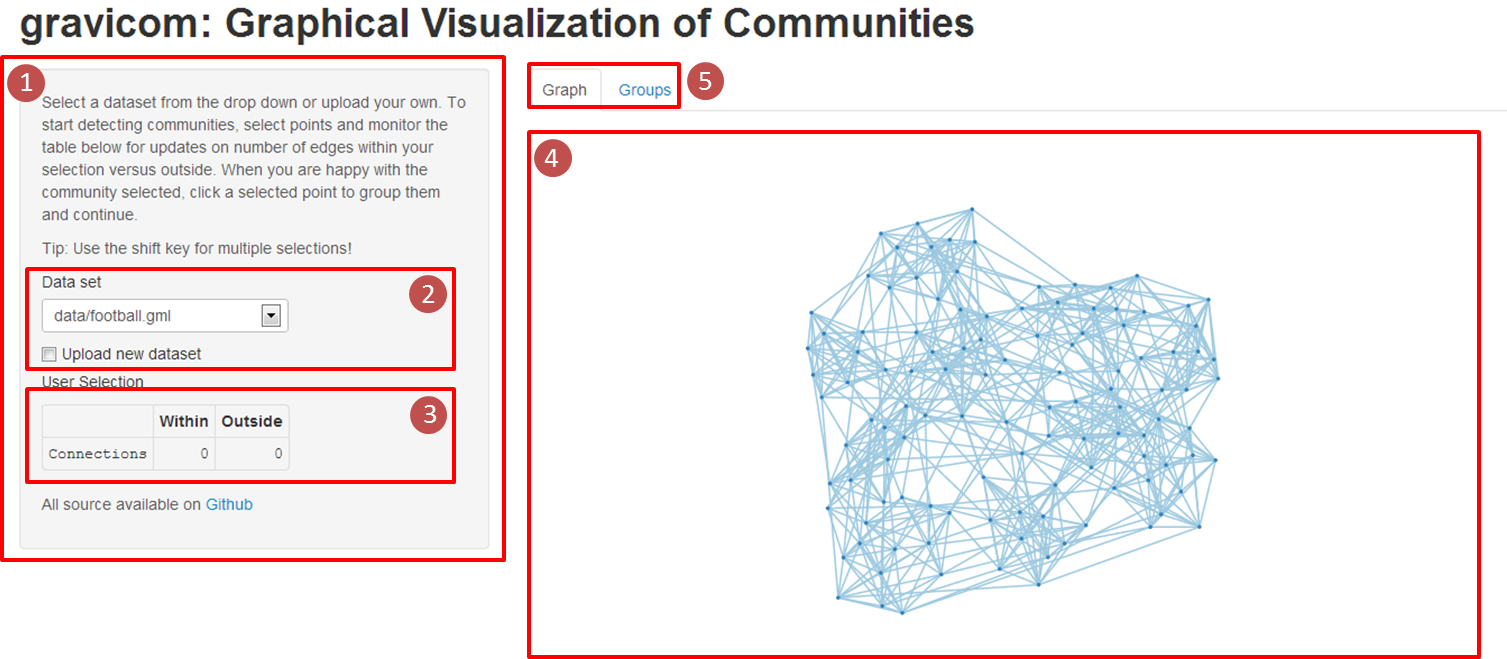
\includegraphics[width=\textwidth]{images/sitecomponents.png}
\caption{\label{fig:sitecomponents} The components that make up gravicom, (1) Control panel, (2) Data management, (3) Connection table, (4) Graph display, and (5) Tabset.}
\end{figure}

Each of these pieces serves as a means for the user to interact with gravicom, either through controls that allow user input to gravicom or through direct interaction with diagnostics and visualization of a graph. Their placement on the gravicom interface can be seen in figure~\ref{fig:sitecomponents}.

\paragraph{Control Panel}
The control panel serves as the starting point for a user's session in gravicom. It contains intructions for the user, as well as the means for a user to select a dataset and the diagnostic connection table. Additionally, the control panel contains a link to the source code for gravicom, should a user be interested in the inner workings of gravicom.

\paragraph{Data Management}
The data management piece is made up of two main parts, data selection and data download. The data selection can be accomplished in two ways, the first being a drop down to select pre-loaded datasets to display. Currently there are two toy datasets in gravicom, a college football dataset and a karate friends dataset. From the dropdown the user can change the dataset to display in the graph. The second part of data selection gives the user the ability to upload his own dataset. Upon clicking the ``Upload new dataset" checkbox, a file selection control appears which gives the user the ability to upload his own graph data to explore with gravicom. This is shown in figure~\ref{fig:uploadnewdataset}. 

\begin{figure}[H]
\centering

\includegraphics[]{images/uploadnewdataset.png}
\caption{\label{fig:uploadnewdataset} The data selection area upon clicking the ``Upload new dataset" checkbox.}
\end{figure}

Data can be downloaded from gravicom with current communities stored. This feature can be used as a save point in working with a graph or as a means to export changes made in gravicom to another tool.



\paragraph{Connection Table}
The connection table is a diagnostic tool for the user to help determine if he has detected a community in his graph. The  table displays the number of connections within a user's selection of nodes in the graph and the number of connections from nodes in a user's selection to nodes not in the selection. The comparison of these two numbers can give the user an idea of if what he has selected is a community or not. The idea behind the connection table is that a community will have more connections within than connections to nodes outside the community.  To aid in the comparison, there is also a proportion column that displays the ratio of number of connections within a selection to the number of connections outside the selection. 

\paragraph{Graph Display}
The graph display shows an interactive graphical representation of  the selected (or uploaded) graph data. Upon load, the graph displays all nodes and edges in the dataset using a force-directed layout algorithm. The user has several ways to interact with the graph: drag, select, and group. A user can drag a node at any time. % to attempt to get a better view of potential communities. However, the graph is setup with a gravity parameter that generally keeps the graph in the center of the screen. 
Upon dragging, the force-directed layout is  rerun, giving an altered view of the graph. Figure~\ref{fig:graphdrag} shows a graph in the process of being dragged.

\begin{figure}[H]
\centering
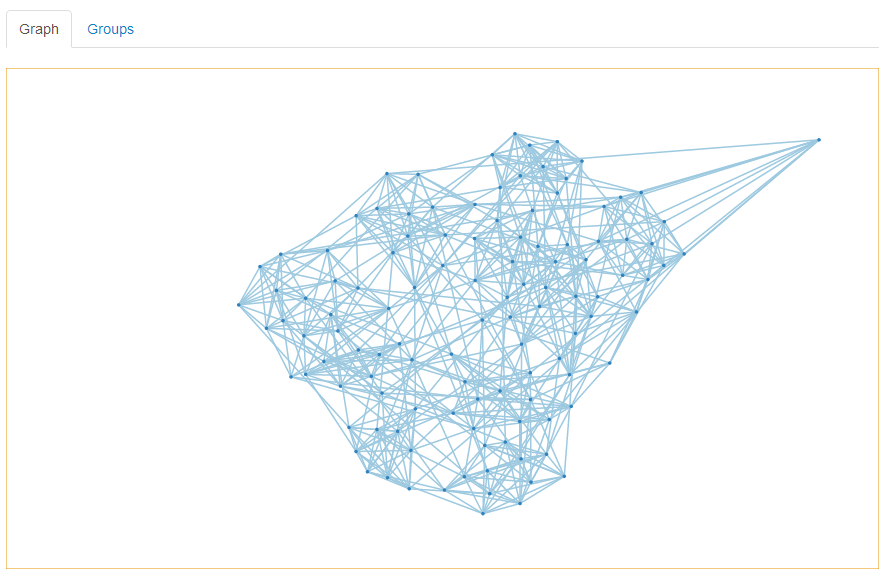
\includegraphics[width=\textwidth]{images/graphdrag.png}
\caption{\label{fig:graphdrag} A graph in the process of being dragged. The node being dragged is marked by a red circle.}
\end{figure}

Selection and grouping of  nodes are actions working together: in order to group nodes, a user  first selects a community based on a visual appraisal of the graph. To select nodes the user clicks and drags a selection box around nodes. See figure~\ref{fig:graphselect} for the results of selection in the interface. The shift key can also be used for multiple selections. Upon selection, the connection table is updated and the user can evaluate their selection as a community and alter the selection if need be (the shift key selection is very useful in this step).

\begin{figure}[H]
\centering
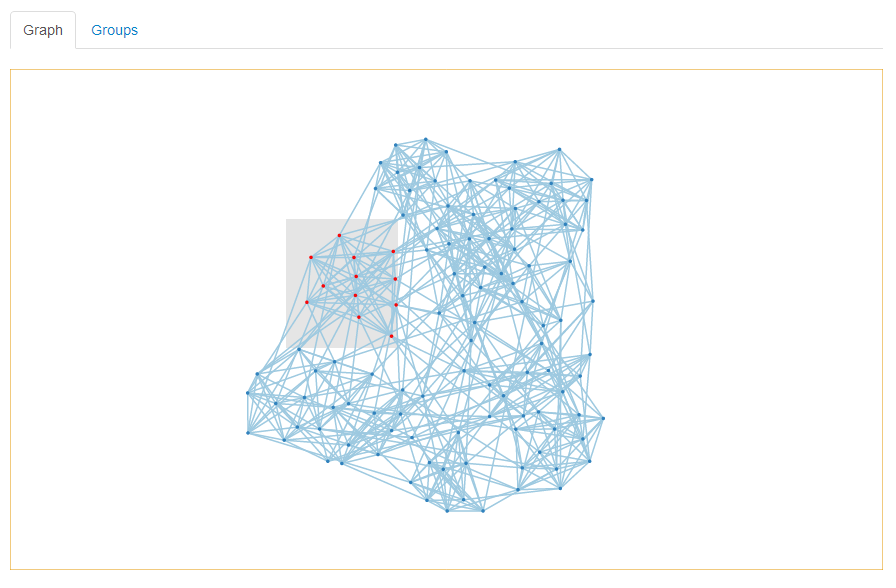
\includegraphics[width=\textwidth]{images/graphselect.png}
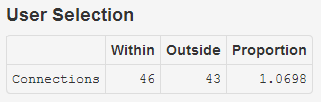
\includegraphics[]{images/tableselect.png}
\caption{\label{fig:graphselect} A graph in the process of nodes being selected. Upon selection of nodes, the connection table updates to display within and outside edges.}
\end{figure}

Selected nodes can be grouped together. Once grouped, a new node is created that comprises all grouped nodes and grouped within edges in size and charge. The force-directed layout is again run, showing the new graph with nodes grouped. This is shown in figure~\ref{fig:graphgroup}. Additionally, grouped nodes are ungrouped by clicking on a grouped node. This process can be repeated until all nodes have been grouped or the user is satisfied that all communities have been detected. 

\begin{figure}[H]
\centering
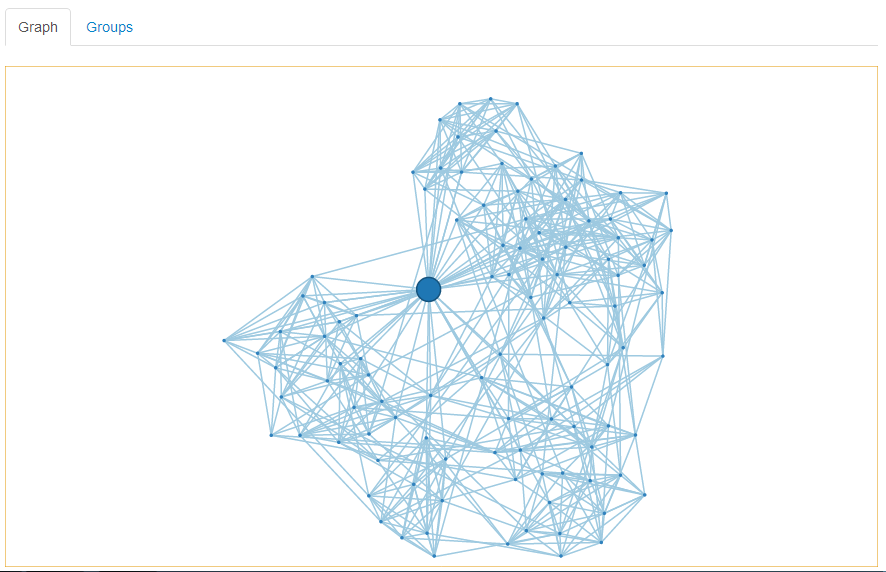
\includegraphics[width=\textwidth]{images/graphgroup.png}
\caption{\label{fig:graphgroup} A graph after nodes have been grouped and the force-directed algorithm has been re-run.}
\end{figure}

\paragraph{Tabset}
The tabset allows the user to switch between two tabs on the screen. The first (and default tab) shows the graph display. The second tab shows the groups that a user has created in the graph. Each group show how many nodes are contained in that group as well as the ability to drop down and view the nodes contained in that group. If the data are equipped with node labels, these will be displayed. If there are no node labels provided, node IDs will be shown. For an example, see figure~\ref{fig:groupstab}.

\begin{figure}[H]
\centering
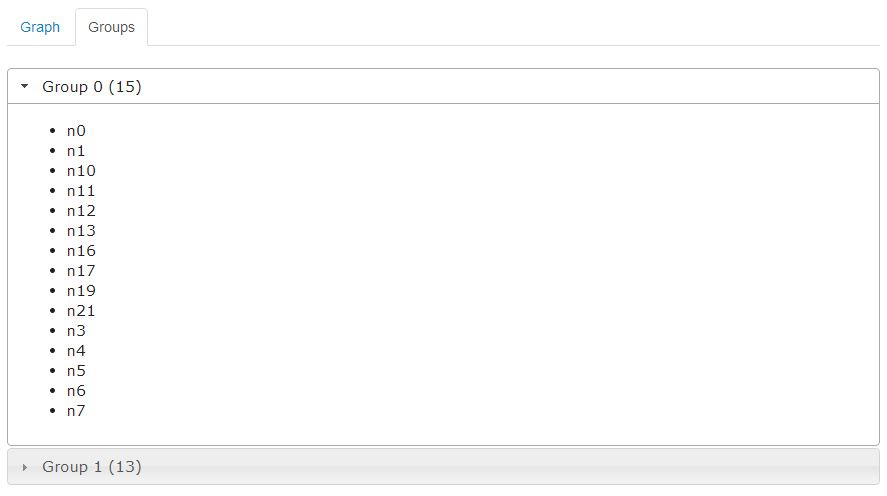
\includegraphics[width=\textwidth]{images/groupstab.png}
\caption{\label{fig:groupstab} The groups tabset displaying which nodes have been grouped in Group 0, for example. The groups tabset also shows that Group 0 has 15 nodes, while Group 1 has 13 nodes.}
\end{figure}


\subsection{Examples}










